\section{Simplicial Homotopies}

\subsection{Homotopies of Morphisms}

For any $\infty$-category, there is the notion of homotopy between morphisms, which can be visualized using $2$-simplices.

\begin{definition}[Homotopy of Morphism]
	Let $\C$ be an $\infty$-category, and $f, g: X \to Y$ be two morphisms in $C$, i.e., $f, g \in \C_1$.
	If $d_1f = d_1g$, and there exists a $2$-simplex $\sigma \in C_2$ such that we have the following diagram
	$$
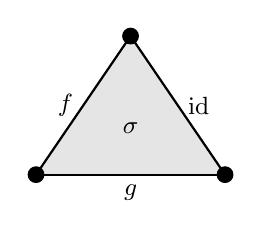
\begin{tikzpicture}[line cap=round, font=\small, scale=0.8]

  % coordinates
  \coordinate (L) at (0,0);
  \coordinate (R) at (3,0);
  \coordinate (T) at (1.5,2.2);
  % \node at ($(L)+(R)+(T)/3$) {$\sigma$};

  % shaded triangle
  \fill[gray!20] (L) -- (R) -- (T) -- cycle;

  % edges
  \draw[thick] (L) -- node[midway, below] {$g$} (R);
  \draw[thick] (L) -- node[midway, left] {$f$} (T);
  \draw[thick] (T) -- node[midway, right] {id} (R);

  % vertices
  \foreach \p in {L,R,T}
    \node[draw, fill, circle, inner sep=2pt] at (\p) {};

	\node at (barycentric cs:L=1,R=1,T=1) {$\sigma$};
\end{tikzpicture}
$$
then we say $f$ is \emph{homotopic} to $g$, denoted as $f \simeq g$.
\end{definition}

\begin{lemma}
In an $\infty$-category $\C$ if we have morphism $f, g$ and $h =  f \circ g$ and $h' = f\circ g$, then $h \simeq h'$.
\end{lemma}


\begin{proof}
The key observation is that we can use the inner horn-filling condition to fill the 3-simplex with vertices $0, 1, 2, 3$ as shown below to demonstrate the homotopy between $h$ and $h'$.
	% demonstration of composition
	$$
\begin{tikzpicture}[font=\small, line cap=round, line join=round]

  % coordinates (adjust to taste)
  \coordinate (v0) at (0,0);      % vertex 0 (left)
  \coordinate (v1) at (1.1,-0.6); % vertex 1 (bottom)
  \coordinate (v2) at (3.2,0);    % vertex 2 (right)
  \coordinate (v3) at (1.7,2.1);  % vertex 3 (top)

  % shades (monochrome)
  \def\shadeA{gray!20}  % left-top
  \def\shadeB{gray!12}  % right
  \def\shadeC{gray!8}   % bottom-left

  % filled triangles (drawn before outlines)
  \fill[\shadeA] (v0) -- (v3) -- (v1) -- cycle; % left-top triangle
  \fill[\shadeB] (v1) -- (v3) -- (v2) -- cycle; % right triangle
  \fill[\shadeC] (v0) -- (v1) -- (v2) -- cycle; % bottom triangle (overlaps intentionally)

  % bold outer edges & internal edges
  \draw[line width=0.9pt] (v0) -- (v3) -- (v2) -- (v1) -- cycle;
  % ensure important diagonals / internal edges are drawn
  \draw[line width=0.9pt] (v0) -- (v1);
  \draw[line width=0.9pt] (v1) -- (v3);
  \draw[line width=0.9pt] (v0) -- (v2);

  % draw vertices as filled dots
  \foreach \p in {v0,v1,v2,v3}
   \node[draw,fill=black,inner sep=1.8pt,circle] at (\p) {};

  % vertex labels (numbers)
  \node[above=2pt] at (v3) {$3$};
  \node[left=2pt]  at (v0) {$0$};
  \node[below=2pt] at (v1) {$1$};
  \node[right=2pt] at (v2) {$2$};

  % edge labels (place them near the middle of corresponding edges)
  \node[left=2pt]  at ($(v0)!0.5!(v1)$) {$f$};
  \node[below=2pt] at ($(v1)!0.5!(v2)$) {$g$};
  \node[above left=2pt] at ($(v0)!0.45!(v3)$) {$h$};
  \node[above right=2pt] at ($(v3)!0.55!(v2)$) {id};

  % central small label h' placed near the small central region
  \node at ($0.28*(v0)+0.34*(v1)+0.38*(v2)$) {$h'$};

  % label g inside the right triangle nearer to top edge
  \node at ($0.6*(v3)+0.25*(v1)+0.15*(v2)$) {$g$};
\end{tikzpicture}
$$
\end{proof}

\begin{definition}[Homotopy Category]
	Let $\C$ be an $\infty$-category. The \emph{homotopy category} $\mathrm{h}\C$ of $\C$ is defined as follows.
	\begin{enumerate}
		\item The objects of $\mathrm{h}\C$ are the same as those of $\C$.
		\item The morphisms in $\mathrm{h}\C$ are given by the equivalence classes of morphisms in $\C$ under the homotopy relation. That is, for objects $X, Y \in \C$, the morphisms from $X$ to $Y$ in $\mathrm{h}\C$ are given by
			$$
			\mathrm{Hom}_{\mathrm{h}\C}(X, Y) := \mathrm{Hom}_{\C}(X, Y) / \simeq,
			$$
			where $\simeq$ denotes the homotopy equivalence relation.
		\item The composition of morphisms in $\mathrm{h}\C$ is induced by the composition in $\C$, and is well-defined due to the lemma above.
	\end{enumerate}
\end{definition}

\subsection{Simplicial Homotopies}

Simplicial sets are equipped with a richer structure that allows us to define homotopies between simplicial maps.

\begin{definition}[Simplicial Homotopy]
	Simplicial Homotopy between two simplicial maps $f, g: X \rightarrow Y$ is defined as a $1$-simplex in the mapping simplicial set $\HomU(X, Y)$,
	$$	H: X \times \Delta^1 \rightarrow Y $$
	such that we have the following commutative diagram
$$
	\begin{tikzcd}[row sep=36pt, column sep=60pt, ampersand replacement=\&]
X\times\Delta^{0}=X
  \arrow[d,"1\times d^{1}"']
  \arrow[dr,"f"]
\& \\
X\times\Delta^{1}
  \arrow[r,"H"]
\& Y \\
X\times\Delta^{0}=X
  \arrow[u,"1\times d^{0}"]
  \arrow[ur,"g"']
\&
\end{tikzcd}
$$

This is equivalent to saying that for each $n$-simplex $x \in X_n$, the image $H(x, -): \Delta^1 \rightarrow Y$ is a $1$-simplex in $Y$ with $d_1H(x, -) = f(x)$ and $d_0H(x, -) = g(x)$.

\end{definition}

Using this, let us demonstrate that simplicial sets are enriched over themselves.

\begin{definition}[Mapping Simplicial Sets]
	For any two simplicial sets $X$ and $Y$, we can define a \emph{mapping simplicial set} $\HomU(X, Y)$ as follows.
	\begin{enumerate}
		\item The $n$-simplices $\HomU(X, Y)_n := \HomU(X, Y)[n] = \hom_{\sS}(X\times \Delta^n, Y)$. 
			Where $X \times \Delta^n$ is the product of simplicial sets defined in \ref{defi:prod-simp}.
		\item For each $\sigma: [m] \rightarrow [n]$, the induced map sends $f: X\Delta^n \rightarrow  Y$ to the composition
			$$
			X \times \Delta^m \xrightarrow{\text{id}_X \times \sigma} X \times \Delta^n \xrightarrow{f} Y.
			$$
	\end{enumerate}
\end{definition}


We define simpicial category as a category enriched over simplicial sets.
\begin{definition}[Simplicial Category]
	A \emph{simplicial category} $\mathcal{C}$ is a category enriched over the category of simplicial sets $\sS$.

	Denote the collection of all simplicial categories as $\textbf{sCat}$.
\end{definition}

Let $J$ be a finite non-empty linearly ordered set. 
We can define a simplicial category $\mathfrak{C}[J]$ as follows: 
\begin{enumerate}
	\item The objects of $\mathfrak{C}[J]$ are the elements of $J$.
	\item For each pair of objects $i, j \in J$, the mapping simplicial set $\mathrm{Map}_{\mathfrak{C}[J]}(i, j)$ is defined as follows:
		\begin{itemize}
			\item If $i > j$, then $\mathrm{Map}_{\mathfrak{C}[J]}(i, j) = \emptyset$ (the empty simplicial set).
			\item If $i \leq j$, then $\mathrm{Map}_{\mathfrak{C}[J]}(i, j)$ is the nerve of the poset of all subsets $I \subseteq J$ such that $i, j \in I$ and for all $k \in I$, we have $i \leq k \leq j$. The ordering is given by inclusion of subsets.
		\end{itemize}
	\item The composition maps
		$$
		\mathrm{Map}_{\mathfrak{C}[J]}(j, k) \times \mathrm{Map}_{\mathfrak{C}[J]}(i, j) \rightarrow \mathrm{Map}_{\mathfrak{C}[J]}(i, k)
		$$
		are induced by the union of subsets.
\end{enumerate}


$\mathfrak{C}$ actually defines a functor from the category of simplicial sets to the category of simplicial categories 
\begin{align*}
	\mathfrak{C}&: \sS \rightarrow \textbf{sCat} \\
	\Delta^{n} &\mapsto \mathfrak{C}[\Delta^{n}]
\end{align*}

If $\C$ is a simplicial category, we can define its simplicial \emph{nerve} (or homotopy coherent nerve) $N(\C)$ as follows:
\begin{definition}[Simplicial Nerve]
	The \emph{simplicial nerve} $N(\C)$ of a simplicial category $\C$ is the simplicial set defined by the formula
	$$
	\hom_{\sS}(\Delta^n, N(\C)) := \hom_{\textbf{sCat}}(\mathfrak{C}[\Delta^n], \C).
	$$
\end{definition}

Lurie showed the following proposition.
\begin{proposition}
	Let $\C$ be a simplicial category such that for every pair of objects $X, Y \in \C$, the mapping simplicial set $\mathrm{Map}_{\C}(X, Y)$ is a Kan complex. Then the simplicial nerve $N(\C)$ is an $\infty$-category.
\end{proposition}

We know that simplicial sets are enriched over themselves. 
Moreover, if we restrict to the full subcategory of simplicial sets consisting of Kan complexes, denoted as $\textbf{Kan}$, then $\textbf{Kan}$ is a simplicial category where the mapping simplicial sets are also Kan complexes.
So Lurire's proposition implies that the simplicial nerve $N(\textbf{Kan})$ is an $\infty$-category.'
